\subsubsection{Apartment-monitor}

\begin{center}
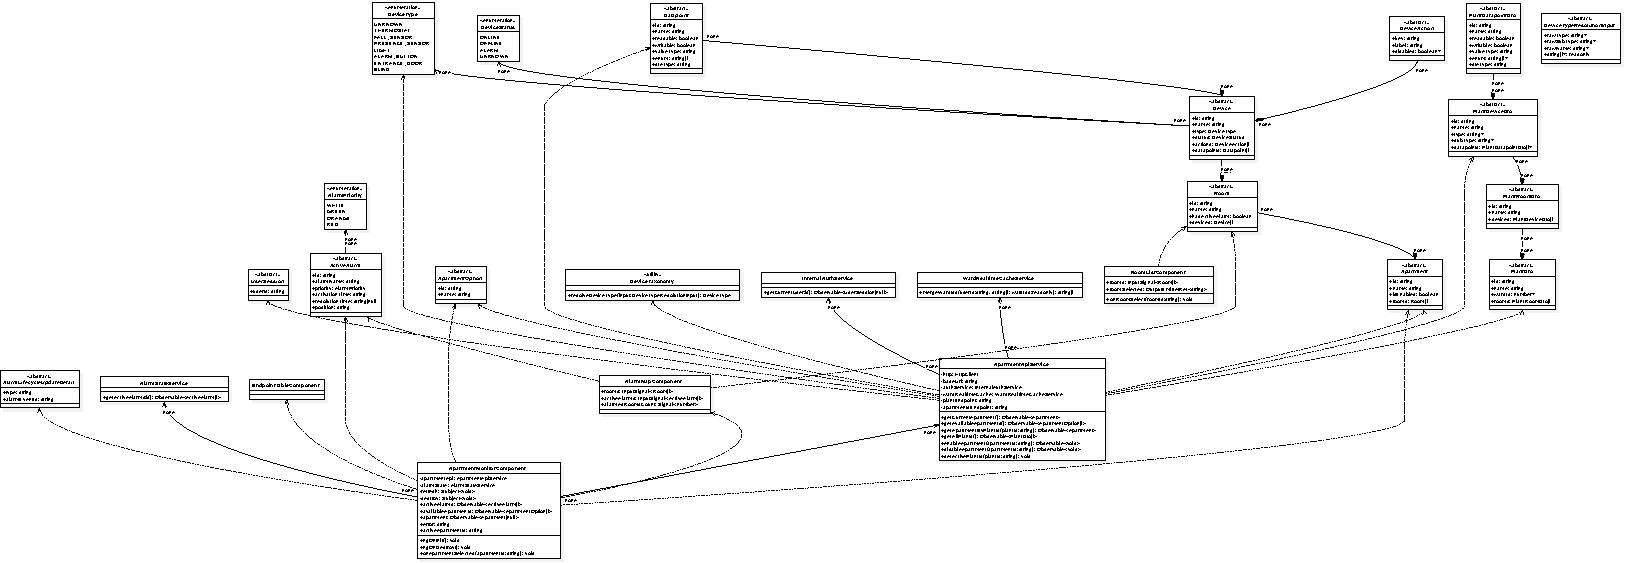
\includegraphics[width=\textwidth]{./frontend/apartment-monitor/apartment-monitor.pdf}
\captionof{figure}{Diagramma delle classi del modulo Apartment monitor}
\end{center}


\addAtr{-}{apartmentApi: ApartmentApiService}{Servizio utilizzato per recuperare e impostare i dati relativi agli appartamenti.}
\addAtr{-}{alarmState: AlarmStateService}{Servizio utilizzato per ottenere lo stato degli allarmi attivi.}
\addAtr{-}{refresh\$: Subject$<$void$>$}{Subject utilizzato per innescare il ricaricamento dei dati dell'appartamento corrente.}
\addAtr{-}{destroy\$: Subject$<$void$>$}{Subject utilizzato per gestire la terminazione delle sottoscrizioni al momento della distruzione del componente.}
\addAtr{+}{activeAlarms\$: Observable$<$Alarm[]$>$}{Stream reattivo che emette la lista degli allarmi attivi, restituendo un array vuoto in assenza di dati.}
\addAtr{+}{availableApartments\$: Observable$<$ApartmentOption[]$>$}{Stream reattivo che emette la lista degli appartamenti disponibili, restituendo un array vuoto in caso di errore.}
\addAtr{+}{apartment\$: Observable$<$Apartment $|$ null$>$}{Stream reattivo che emette i dati dell'appartamento corrente ad ogni refresh, restituendo \texttt{null} in caso di errore.}
\addAtr{+}{error: string}{Messaggio di errore da visualizzare all'utente in caso di fallimento nel caricamento dei dati.}
\addAtr{+}{activeApartmentId: string}{Identificativo dell'appartamento attualmente selezionato.}
\addMet{+}{ngOnInit() : void}{Inizializza la sottoscrizione agli eventi real-time di aggiornamento del ciclo di vita degli allarmi, innescando il refresh dei dati al loro arrivo.}
\addMet{+}{ngOnDestroy() : void}{Completa il Subject \texttt{destroy\$} per terminare tutte le sottoscrizioni attive e prevenire memory leak.}
\addMet{+}{onApartmentSelected(apartmentId: string) : void}{Gestisce la selezione di un nuovo appartamento, impostando l'appartamento attivo tramite l'API e innescando il refresh dei dati.}
\makeCl{ApartmentMonitorComponent}{Componente Angular per il monitoraggio di un appartamento, che visualizza gli allarmi attivi e i dati dell'appartamento corrente. Gestisce la selezione dell'appartamento attivo e si aggiorna in risposta agli eventi real-time di allarme.}

\addAtr{+}{rooms: InputSignal$<$Room[]$>$}{}
\addAtr{+}{activeAlarms: InputSignal$<$ActiveAlarm[]$>$}{}
\addAtr{+}{alarmedRoomsCount: Signal$<$number$>$}{}
\makeCl{AlarmMapComponent}{Componente Angular che visualizza una mappa delle stanze con evidenza di quelle in stato di allarme. Calcola dinamicamente il numero di stanze con allarme attivo tramite un segnale derivato.}

\addAtr{+}{rooms: InputSignal$<$Room[]$>$}{Segnale di input contenente la lista delle stanze da visualizzare, con array vuoto come valore di default.}
\addAtr{+}{roomSelected: OutputEmitterRef$<$string$>$}{Evento emesso quando l'utente seleziona una stanza, contenente l'identificativo della stanza selezionata.}
\addMet{+}{onRoomSelect(roomId: string) : void}{Emette l'evento \texttt{roomSelected} con l'identificativo della stanza selezionata.}
\makeCl{RoomListComponent}{Componente Angular che visualizza la lista delle stanze disponibili. Emette un evento alla selezione di una stanza, comunicando il relativo identificativo al componente padre.}

\addAtr{+}{id: string}{}
\addAtr{+}{name: string}{}
\addAtr{+}{isEnabled: boolean}{}
\addAtr{+}{rooms: Room[]}{}
\makeAbCl{Apartment}{Interfaccia che rappresenta il modello di dominio di un appartamento. Aggrega le informazioni identificative, lo stato di abilitazione e la lista delle stanze.}

\addAtr{+}{id: string}{}
\addAtr{+}{name: string}{}
\addAtr{+}{readable: boolean}{}
\addAtr{+}{writable: boolean}{}
\addAtr{+}{valueType: string}{}
\addAtr{+}{enum: string[]}{}
\addAtr{+}{sfeType: string}{}
\makeAbCl{Datapoint}{Interfaccia che rappresenta un datapoint di un dispositivo. Definisce le proprietà di lettura, scrittura, tipo di valore e valori enumerati disponibili.}

\addAtr{+}{key: string}{}
\addAtr{+}{label: string}{}
\addAtr{+}{disabled?: boolean}{}
\makeAbCl{DeviceAction}{Interfaccia che rappresenta un'azione eseguibile su un dispositivo. Associa una chiave identificativa a un'etichetta visualizzabile e a un flag opzionale di disabilitazione.}

\addAtr{+}{id: string}{}
\addAtr{+}{name: string}{}
\addAtr{+}{type: DeviceType}{}
\addAtr{+}{status: DeviceStatus}{}
\addAtr{+}{actions: DeviceAction[]}{}
\addAtr{+}{datapoints: Datapoint[]}{}
\makeAbCl{Device}{Interfaccia che rappresenta il modello di dominio di un dispositivo. Raccoglie tipo, stato, azioni disponibili e datapoint associati.}

\addAtr{+}{id: string}{}
\addAtr{+}{name: string}{}
\addAtr{+}{readable: boolean}{}
\addAtr{+}{writable: boolean}{}
\addAtr{+}{valueType: string}{}
\addAtr{+}{enum?: string[]}{}
\addAtr{+}{sfeType: string}{}
\makeAbCl{PlantDatapointDto}{Interfaccia che rappresenta il DTO di un datapoint restituito dal backend nella risposta dell'impianto.}

\addAtr{+}{id: string}{}
\addAtr{+}{name: string}{}
\addAtr{+}{type?: string}{}
\addAtr{+}{subType?: string}{}
\addAtr{+}{datapoints?: PlantDatapointDto[]}{}
\makeAbCl{PlantDeviceDto}{Interfaccia che rappresenta il DTO di un dispositivo restituito dal backend nella risposta dell'impianto.}

\addAtr{+}{id: string}{}
\addAtr{+}{name: string}{}
\addAtr{+}{devices: PlantDeviceDto[]}{}
\makeAbCl{PlantRoomDto}{Interfaccia che rappresenta il DTO di una stanza restituita dal backend nella risposta dell'impianto.}

\addAtr{+}{id: string}{}
\addAtr{+}{name: string}{}
\addAtr{+}{wardId?: number}{}
\addAtr{+}{rooms: PlantRoomDto[]}{}
\makeAbCl{PlantDto}{Interfaccia che rappresenta il DTO di un impianto restituito dal backend, contenente le stanze e l'eventuale identificativo del ward associato.}

\addAtr{+}{id: string}{}
\addAtr{+}{name: string}{}
\addAtr{+}{hasActiveAlarm: boolean}{}
\addAtr{+}{devices: Device[]}{}
\makeAbCl{Room}{Interfaccia che rappresenta il modello di dominio di una stanza. Aggrega le informazioni identificative, lo stato di allarme attivo e la lista dei dispositivi presenti.}

\addAtr{-}{http: HttpClient}{Client HTTP utilizzato per effettuare le richieste alle API REST.}
\addAtr{-}{baseUrl: string}{URL base dell'API, iniettato tramite token \texttt{API\_BASE\_URL}.}
\addAtr{-}{authService: InternalAuthService}{Servizio di autenticazione utilizzato per recuperare l'utente corrente.}
\addAtr{-}{wardRealtimeCache: WardRealtimeCacheService}{Servizio utilizzato per aggiornare la cache degli identificativi dei ward associati all'utente corrente.}
\addAtr{-}{plantEndpoint: string}{URL dell'endpoint per le operazioni sugli impianti.}
\addAtr{-}{apartmentsEndpoint: string}{URL dell'endpoint per le operazioni sugli appartamenti.}
\addMet{+}{getCurrentApartment() : Observable$<$Apartment$>$}{Recupera l'appartamento corrente selezionando l'impianto attivo tra quelli disponibili e caricandone i dettagli.}
\addMet{+}{getAvailableApartments() : Observable$<$ApartmentOption[]$>$}{Restituisce la lista degli appartamenti disponibili ordinata alfabeticamente per nome.}
\addMet{+}{getApartmentByPlantId(plantId: string) : Observable$<$Apartment$>$}{Recupera i dettagli dell'appartamento associato all'identificativo di impianto specificato.}
\addMet{+}{getAllPlants() : Observable$<$PlantDto[]$>$}{Recupera tutti gli impianti disponibili dal backend e aggiorna la cache dei ward per l'utente corrente.}
\addMet{+}{enableApartment(apartmentId: string) : Observable$<$void$>$}{Invia una richiesta PATCH per abilitare l'appartamento con l'identificativo specificato.}
\addMet{+}{disableApartment(apartmentId: string) : Observable$<$void$>$}{Invia una richiesta PATCH per disabilitare l'appartamento con l'identificativo specificato.}
\addMet{+}{setActivePlantId(plantId: string) : void}{Salva l'identificativo dell'impianto attivo nel localStorage e dispatcha un evento custom se il valore è cambiato.}
\addMet{-}{getActivePlantId() : string $|$ null}{Recupera l'identificativo dell'impianto attivo dal localStorage, restituendo \texttt{null} se non disponibile.}
\addMet{-}{getAvailablePlants() : Observable$<$PlantDto[]$>$}{Delega il recupero degli impianti disponibili al metodo \texttt{getAllPlants}.}
\addMet{-}{extractPlants(response: unknown) : PlantDto[]}{Estrae l'array di impianti da una risposta generica del backend, gestendo sia array diretti che oggetti con proprietà \texttt{data} o \texttt{plants}.}
\addMet{-}{asPlantArray(value: unknown) : PlantDto[]}{Converte un valore generico in un array di \texttt{PlantDto} validi, deduplicando per identificativo e normalizzando il nome.}
\addMet{-}{cacheWardIdsForCurrentUser(plants: ReadonlyArray$<$PlantDto$>$) : void}{Estrae gli identificativi dei ward dagli impianti forniti e li memorizza nella cache per l'utente corrente.}
\addMet{-}{mapPlantToApartment(plant: PlantDto) : Apartment}{Trasforma un \texttt{PlantDto} nel modello di dominio \texttt{Apartment}, mappando stanze e dispositivi e filtrando i dispositivi di misura energetica.}
\addMet{-}{deduplicateRoomDevices(devices: ReadonlyArray$<$PlantDeviceDto$>$) : PlantDeviceDto[]}{Deduplica i dispositivi di una stanza per nome normalizzato, mantenendo quello con il punteggio di priorità più alto.}
\addMet{-}{normalizeDeviceName(name: string) : string}{Normalizza il nome di un dispositivo rimuovendo spazi e convertendo in minuscolo.}
\addMet{-}{getDevicePriorityScore(device: PlantDeviceDto) : number}{Calcola un punteggio di priorità per un dispositivo in base al tipo, sottotipo e numero di datapoint.}
\addMet{-}{isEnergyMeasureDevice(rawType: string $|$ undefined, rawSubType: string $|$ undefined) : boolean}{Verifica se un dispositivo è di tipo misura energetica in base al tipo e sottotipo forniti.}
\addMet{-}{mapDeviceStatus(rawType: string $|$ undefined) : DeviceStatus}{Mappa il tipo grezzo di un dispositivo nel corrispondente stato, restituendo \texttt{ONLINE} se il tipo è definito, \texttt{UNKNOWN} altrimenti.}
\makeCl{ApartmentApiService}{Servizio Angular per la gestione delle chiamate API relative agli appartamenti e agli impianti. Espone operazioni per il recupero, la selezione e l'abilitazione degli appartamenti, gestendo internamente la mappatura dei dati e la cache dei ward.}